% Move red left, harder case: flip, rotate right at h.right, rotate left at h, then flip.
% Editable source for this diagram. From this directory, regenerate with:
% latex -interaction=nonstopmode -halt-on-error llrbt-8.tex
% dvisvgm --no-fonts --exact --bbox=papersize --output=llrbt-8.svg llrbt-8.dvi
\documentclass[tikz,border=12pt]{standalone}
\usepackage{lmodern}
\usepackage{tikz}
\usetikzlibrary{arrows.meta,backgrounds,shapes.geometric,patterns}
\definecolor{linkred}{HTML}{B5240A}
\definecolor{noteBlue}{HTML}{0067A5}
\definecolor{softgreen}{HTML}{D8EAD0}
\definecolor{softpurple}{HTML}{D9D1E8}
\definecolor{softpink}{HTML}{F5CECF}
\definecolor{softyellow}{HTML}{FFF2C9}
% Translucent vector layers keep the soft shadow in the DVI-to-SVG export.
\tikzset{
  llrbt shadow layer/.style args={#1/#2}{
    preaction={fill=black,draw=none,fill opacity=#2,
      transform canvas={shift={(3pt,-3pt)},
        scale around=#1:(current path bounding box.center)}}
  },
  llrbt shadow/.style={
    llrbt shadow layer=1.40/0.01,
    llrbt shadow layer=1.35/0.015,
    llrbt shadow layer=1.30/0.025,
    llrbt shadow layer=1.25/0.04,
    llrbt shadow layer=1.20/0.06,
    llrbt shadow layer=1.15/0.08,
    llrbt shadow layer=1.10/0.10,
    llrbt shadow layer=1.05/0.12,
    llrbt shadow layer=1.00/0.14,
    llrbt shadow layer=0.95/0.16,
    llrbt shadow layer=0.90/0.18,
    llrbt shadow layer=0.85/0.20
  }
}
\begin{document}
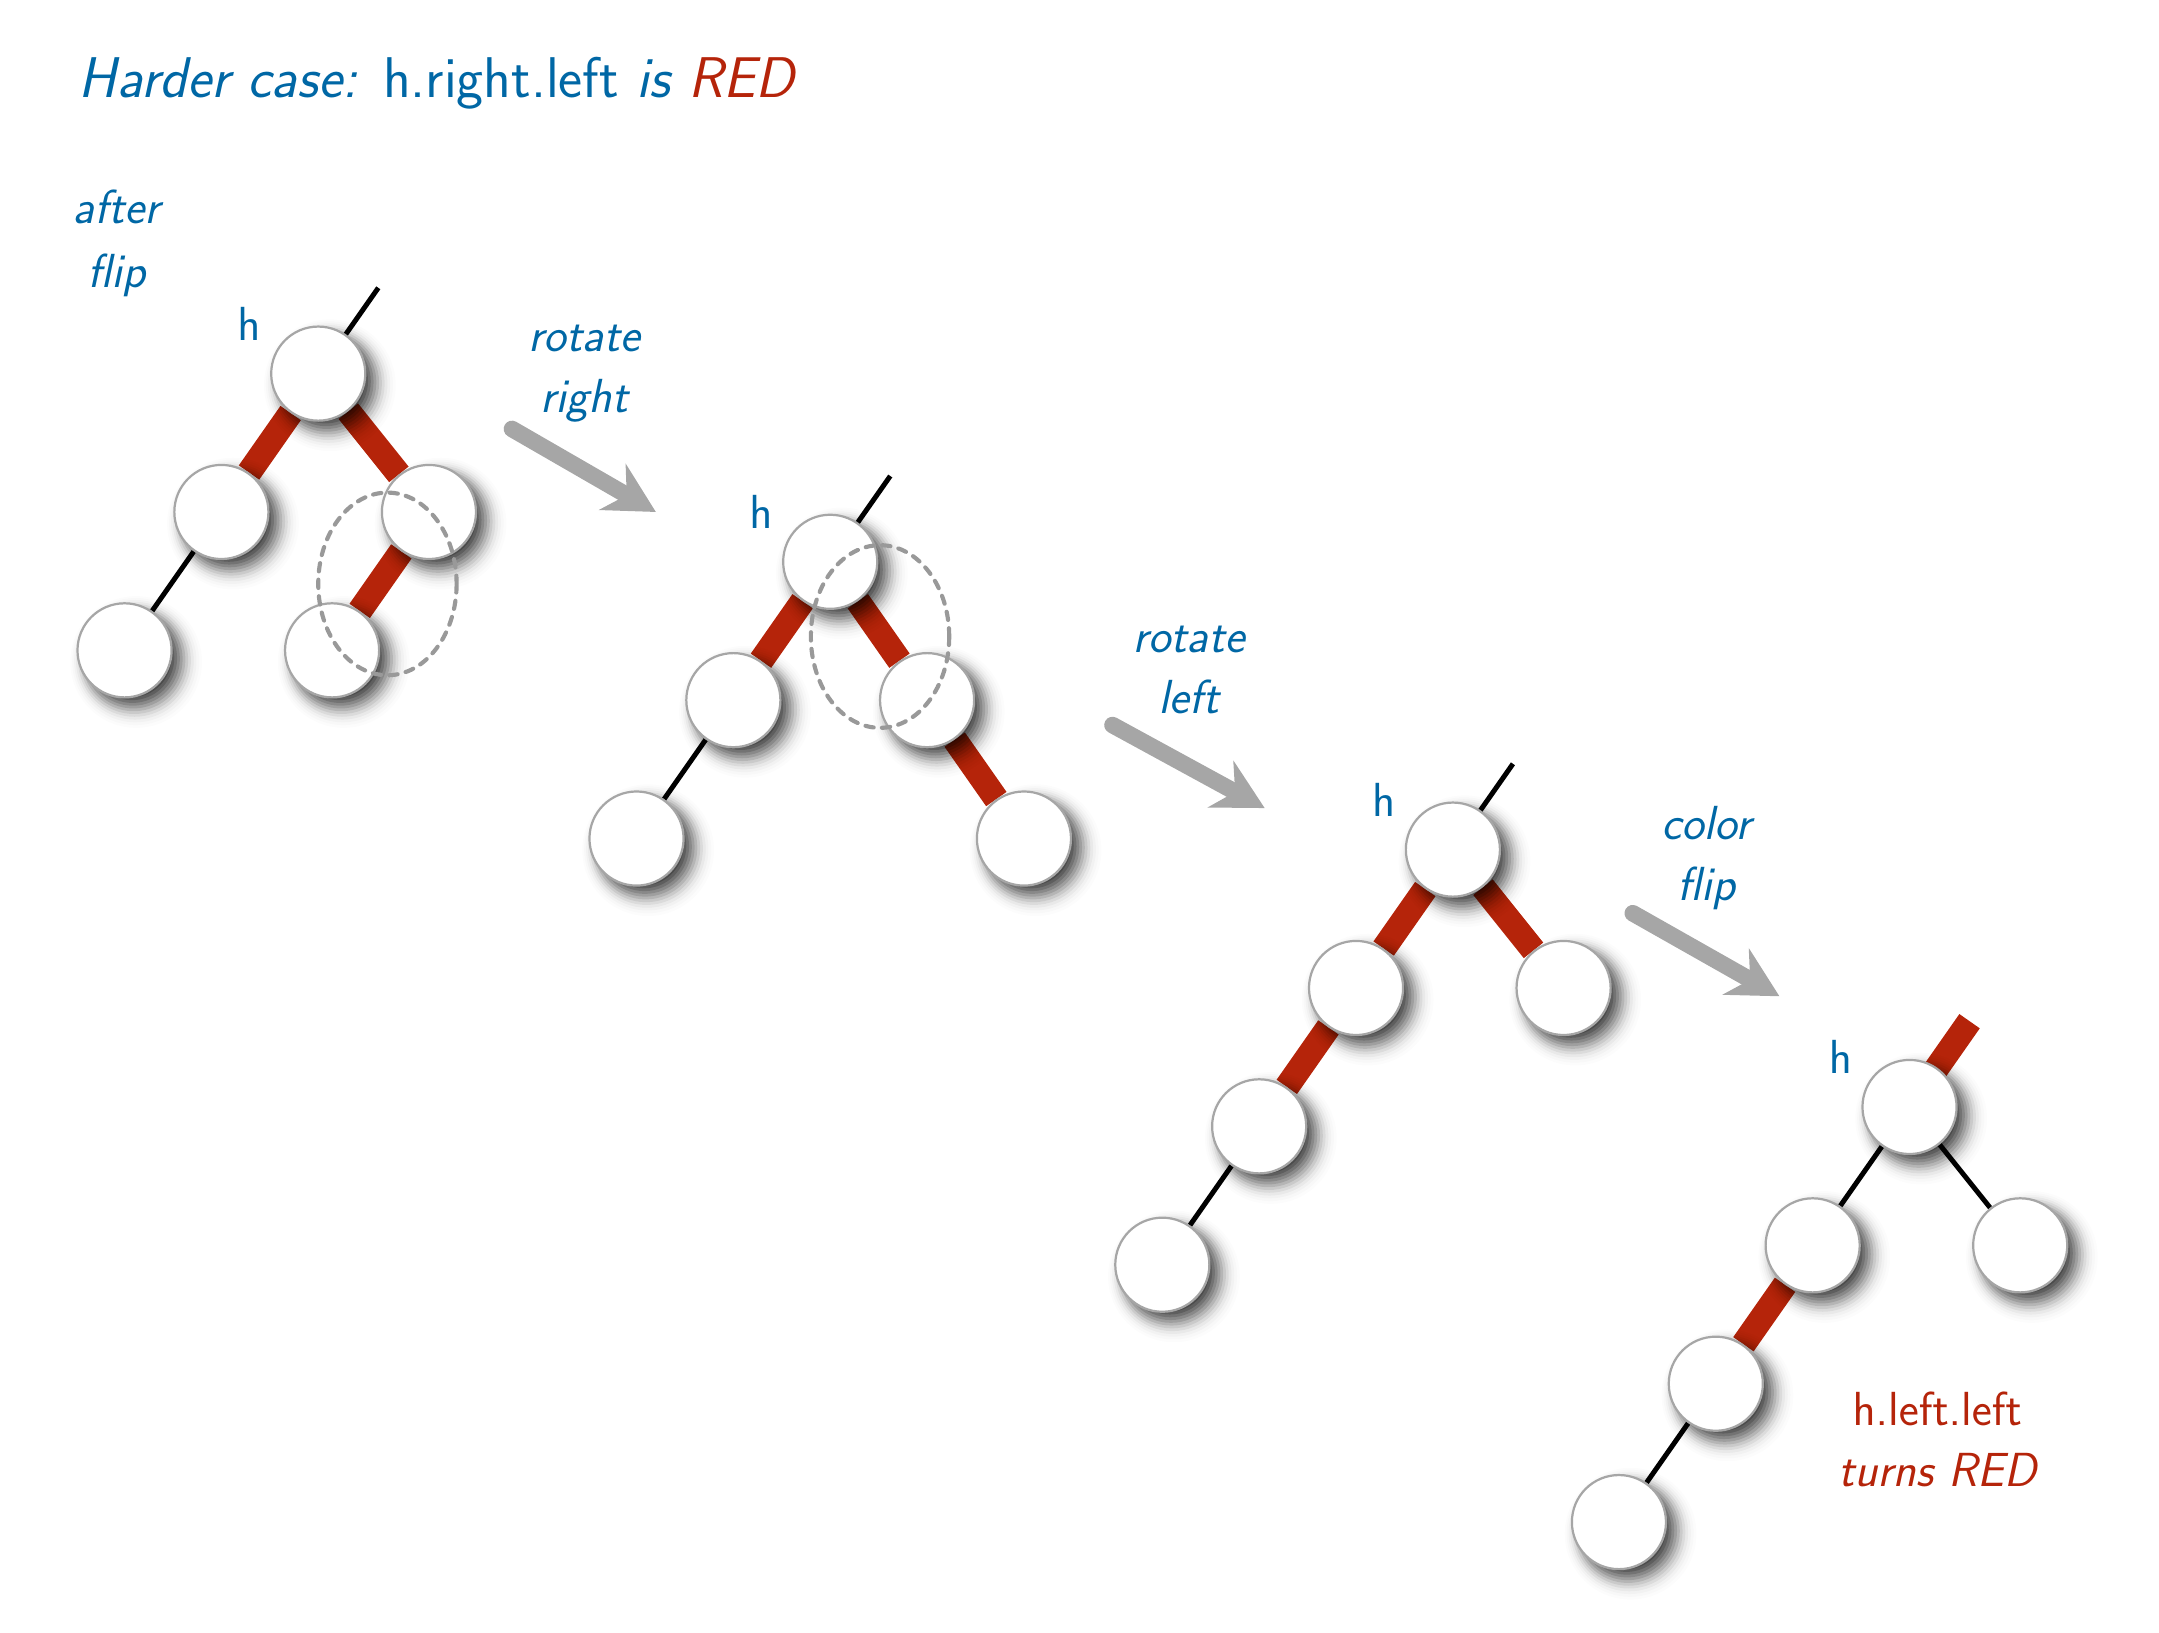
\begin{tikzpicture}[x=1pt,y=-1pt,>=Stealth,line cap=round,line join=round]
\path[use as bounding box] (0,0) rectangle (760,570);
\begin{scope}[on background layer]
\draw[draw=black,line width=1.8pt] (105,125) -- (126.7,94);
\draw[draw=black,line width=1.8pt] (290,193) -- (311.7,162);
\draw[draw=black,line width=1.8pt] (515,297) -- (536.7,266);
\draw[draw=linkred,line width=9pt] (680,390) -- (701.7,359);
\end{scope}
\node[llrbt shadow,circle,draw=black!35,fill=white,text=noteBlue,minimum size=34pt,inner sep=0pt,line width=0.8pt,font=\sffamily\fontsize{18}{21.6}\selectfont,font=\sffamily\itshape\fontsize{18}{22}\selectfont] (ah) at (105,125) {};
\node[llrbt shadow,circle,draw=black!35,fill=white,text=noteBlue,minimum size=34pt,inner sep=0pt,line width=0.8pt,font=\sffamily\fontsize{18}{21.6}\selectfont,font=\sffamily\itshape\fontsize{18}{22}\selectfont] (al) at (70,175) {};
\node[llrbt shadow,circle,draw=black!35,fill=white,text=noteBlue,minimum size=34pt,inner sep=0pt,line width=0.8pt,font=\sffamily\fontsize{18}{21.6}\selectfont,font=\sffamily\itshape\fontsize{18}{22}\selectfont] (all) at (35,225) {};
\node[llrbt shadow,circle,draw=black!35,fill=white,text=noteBlue,minimum size=34pt,inner sep=0pt,line width=0.8pt,font=\sffamily\fontsize{18}{21.6}\selectfont,font=\sffamily\itshape\fontsize{18}{22}\selectfont] (ar) at (145,175) {};
\node[llrbt shadow,circle,draw=black!35,fill=white,text=noteBlue,minimum size=34pt,inner sep=0pt,line width=0.8pt,font=\sffamily\fontsize{18}{21.6}\selectfont,font=\sffamily\itshape\fontsize{18}{22}\selectfont] (arl) at (110,225) {};
\node[llrbt shadow,circle,draw=black!35,fill=white,text=noteBlue,minimum size=34pt,inner sep=0pt,line width=0.8pt,font=\sffamily\fontsize{18}{21.6}\selectfont,font=\sffamily\itshape\fontsize{18}{22}\selectfont] (bh) at (290,193) {};
\node[llrbt shadow,circle,draw=black!35,fill=white,text=noteBlue,minimum size=34pt,inner sep=0pt,line width=0.8pt,font=\sffamily\fontsize{18}{21.6}\selectfont,font=\sffamily\itshape\fontsize{18}{22}\selectfont] (bl) at (255,243) {};
\node[llrbt shadow,circle,draw=black!35,fill=white,text=noteBlue,minimum size=34pt,inner sep=0pt,line width=0.8pt,font=\sffamily\fontsize{18}{21.6}\selectfont,font=\sffamily\itshape\fontsize{18}{22}\selectfont] (bll) at (220,293) {};
\node[llrbt shadow,circle,draw=black!35,fill=white,text=noteBlue,minimum size=34pt,inner sep=0pt,line width=0.8pt,font=\sffamily\fontsize{18}{21.6}\selectfont,font=\sffamily\itshape\fontsize{18}{22}\selectfont] (br) at (325,243) {};
\node[llrbt shadow,circle,draw=black!35,fill=white,text=noteBlue,minimum size=34pt,inner sep=0pt,line width=0.8pt,font=\sffamily\fontsize{18}{21.6}\selectfont,font=\sffamily\itshape\fontsize{18}{22}\selectfont] (brr) at (360,293) {};
\node[llrbt shadow,circle,draw=black!35,fill=white,text=noteBlue,minimum size=34pt,inner sep=0pt,line width=0.8pt,font=\sffamily\fontsize{18}{21.6}\selectfont,font=\sffamily\itshape\fontsize{18}{22}\selectfont] (ch) at (515,297) {};
\node[llrbt shadow,circle,draw=black!35,fill=white,text=noteBlue,minimum size=34pt,inner sep=0pt,line width=0.8pt,font=\sffamily\fontsize{18}{21.6}\selectfont,font=\sffamily\itshape\fontsize{18}{22}\selectfont] (cl) at (480,347) {};
\node[llrbt shadow,circle,draw=black!35,fill=white,text=noteBlue,minimum size=34pt,inner sep=0pt,line width=0.8pt,font=\sffamily\fontsize{18}{21.6}\selectfont,font=\sffamily\itshape\fontsize{18}{22}\selectfont] (cll) at (445,397) {};
\node[llrbt shadow,circle,draw=black!35,fill=white,text=noteBlue,minimum size=34pt,inner sep=0pt,line width=0.8pt,font=\sffamily\fontsize{18}{21.6}\selectfont,font=\sffamily\itshape\fontsize{18}{22}\selectfont] (clll) at (410,447) {};
\node[llrbt shadow,circle,draw=black!35,fill=white,text=noteBlue,minimum size=34pt,inner sep=0pt,line width=0.8pt,font=\sffamily\fontsize{18}{21.6}\selectfont,font=\sffamily\itshape\fontsize{18}{22}\selectfont] (cr) at (555,347) {};
\node[llrbt shadow,circle,draw=black!35,fill=white,text=noteBlue,minimum size=34pt,inner sep=0pt,line width=0.8pt,font=\sffamily\fontsize{18}{21.6}\selectfont,font=\sffamily\itshape\fontsize{18}{22}\selectfont] (dh) at (680,390) {};
\node[llrbt shadow,circle,draw=black!35,fill=white,text=noteBlue,minimum size=34pt,inner sep=0pt,line width=0.8pt,font=\sffamily\fontsize{18}{21.6}\selectfont,font=\sffamily\itshape\fontsize{18}{22}\selectfont] (dl) at (645,440) {};
\node[llrbt shadow,circle,draw=black!35,fill=white,text=noteBlue,minimum size=34pt,inner sep=0pt,line width=0.8pt,font=\sffamily\fontsize{18}{21.6}\selectfont,font=\sffamily\itshape\fontsize{18}{22}\selectfont] (dll) at (610,490) {};
\node[llrbt shadow,circle,draw=black!35,fill=white,text=noteBlue,minimum size=34pt,inner sep=0pt,line width=0.8pt,font=\sffamily\fontsize{18}{21.6}\selectfont,font=\sffamily\itshape\fontsize{18}{22}\selectfont] (dlll) at (575,540) {};
\node[llrbt shadow,circle,draw=black!35,fill=white,text=noteBlue,minimum size=34pt,inner sep=0pt,line width=0.8pt,font=\sffamily\fontsize{18}{21.6}\selectfont,font=\sffamily\itshape\fontsize{18}{22}\selectfont] (dr) at (720,440) {};
\begin{scope}[on background layer]
\draw[draw=linkred,line width=9pt] (ah) -- (al);
\draw[draw=black,line width=1.8pt] (al) -- (all);
\draw[draw=linkred,line width=9pt] (ah) -- (ar);
\draw[draw=linkred,line width=9pt] (ar) -- (arl);
\draw[draw=linkred,line width=9pt] (bh) -- (bl);
\draw[draw=black,line width=1.8pt] (bl) -- (bll);
\draw[draw=linkred,line width=9pt] (bh) -- (br);
\draw[draw=linkred,line width=9pt] (br) -- (brr);
\draw[draw=linkred,line width=9pt] (ch) -- (cl);
\draw[draw=linkred,line width=9pt] (cl) -- (cll);
\draw[draw=black,line width=1.8pt] (cll) -- (clll);
\draw[draw=linkred,line width=9pt] (ch) -- (cr);
\draw[draw=black,line width=1.8pt] (dh) -- (dl);
\draw[draw=linkred,line width=9pt] (dl) -- (dll);
\draw[draw=black,line width=1.8pt] (dll) -- (dlll);
\draw[draw=black,line width=1.8pt] (dh) -- (dr);
\end{scope}
\node[anchor=west,text=noteBlue,font=\sffamily\itshape\fontsize{20}{24}\selectfont] at (15,20) {Harder case: \textup{h.right.left} is \textcolor{linkred}{RED}};
\node[anchor=center,text=noteBlue,font=\sffamily\fontsize{19}{22.8}\selectfont,align=center,font=\sffamily\itshape\fontsize{19}{23}\selectfont] at (32,78) {after\\flip};
\node[anchor=center,text=noteBlue,font=\sffamily\fontsize{18}{21.6}\selectfont] at (80,107) {h};
\draw[draw=black!40,dashed,line width=1.5pt] (130,201) ellipse (25pt and 33pt);
\draw[draw=black!35,line width=6pt,->,>={Stealth[length=18pt,width=19pt]}] (175,145) -- (227,175);
\node[anchor=center,text=noteBlue,font=\sffamily\fontsize{18}{21.6}\selectfont,align=center,font=\sffamily\itshape\fontsize{18}{22}\selectfont] at (201.0,125.0) {rotate\\right};
\node[anchor=center,text=noteBlue,font=\sffamily\fontsize{18}{21.6}\selectfont] at (265,175) {h};
\draw[draw=black!40,dashed,line width=1.5pt] (308,220) ellipse (25pt and 33pt);
\draw[draw=black!35,line width=6pt,->,>={Stealth[length=18pt,width=19pt]}] (392,252) -- (447,282);
\node[anchor=center,text=noteBlue,font=\sffamily\fontsize{18}{21.6}\selectfont,align=center,font=\sffamily\itshape\fontsize{18}{22}\selectfont] at (419.5,232.0) {rotate\\left};
\node[anchor=center,text=noteBlue,font=\sffamily\fontsize{18}{21.6}\selectfont] at (490,279) {h};
\draw[draw=black!35,line width=6pt,->,>={Stealth[length=18pt,width=19pt]}] (580,320) -- (633,350);
\node[anchor=center,text=noteBlue,font=\sffamily\fontsize{18}{21.6}\selectfont,align=center,font=\sffamily\itshape\fontsize{18}{22}\selectfont] at (606.5,300.0) {color\\flip};
\node[anchor=center,text=noteBlue,font=\sffamily\fontsize{18}{21.6}\selectfont] at (655,372) {h};
\node[anchor=center,text=linkred,align=center,font=\sffamily\itshape\fontsize{18}{22}\selectfont] at (690,510) {\textup{h.left.left}\\turns RED};
\end{tikzpicture}
\end{document}
